\documentclass{article}
\pdfminorversion=6
\usepackage[utf8]{inputenc}
\usepackage{amssymb, amsmath, amsthm}
\usepackage{thmtools, mathtools, mathrsfs}
\usepackage{amsfonts}
\usepackage{stmaryrd}
\usepackage[sort&compress,numbers]{natbib}
\usepackage{subcaption}
\usepackage{graphicx}
\usepackage{caption}
\usepackage{float}
\usepackage{bm}
\usepackage{tikz}
\usepackage{tikz-cd} 

\newcommand{\defvec}[1]{\expandafter\newcommand\csname v#1\endcsname{{\mathbf{#1}}}}
\newcommand{\dm}[1]{\ensuremath{\mathrm{d}{#1}}} % dx dy dz dmu
\newcommand{\RN}[2]{\frac{\dm{#1}}{\dm{#2}}} % (Radon-Nikodym) derivative
\newcommand{\PD}[2]{\frac{\partial #1}{\partial #2}} % partial derivative
\newcommand{\mb}[1]{\mathbb{#1}}
\newcommand{\mc}[1]{\mathcal{#1}}
\newcommand{\overbar}[1]{\mkern 1.5mu\overline{\mkern-1.5mu#1\mkern-1.5mu}\mkern 1.5mu}
\newcommand{\win}{W_{\text{in}}}
\newcommand{\wout}{W_{\text{out}}}
\newcommand{\bout}{b_{\text{out}}}

\DeclareMathOperator{\Inv}{Inv}
\DeclareMathOperator{\innt}{int}
\DeclareMathOperator{\relu}{ReLU}

% if you need to pass options to natbib, use, e.g.:
%     \PassOptionsToPackage{numbers, compress}{natbib}
% before loading neurips_2023

% ready for submission
% \usepackage{neurips_2023}

% to compile a preprint version, e.g., for submission to arXiv, add the
% [preprint] option:
%     \usepackage[preprint]{neurips_2023}

% to compile a camera-ready version, add the [final] option, e.g.:
%     \usepackage[final]{neurips_2023}

% to avoid loading the natbib package, add option nonatbib:
     \usepackage[]{neurips_2023}
     
\usepackage[utf8]{inputenc} % allow utf-8 input
\usepackage[T1]{fontenc}    % use 8-bit T1 fonts
\usepackage{hyperref}       % hyperlinks
\usepackage{url}            % simple URL typesetting
\usepackage{booktabs}       % professional-quality tables
\usepackage{amsfonts}       % blackboard math symbols
\usepackage{nicefrac}       % compact symbols for 1/2, etc.
\usepackage{microtype}      % microtypography

\newcommand{\probP}{\text{I\kern-0.15em P}}

\newtheorem{theorem}{Theorem}
\newtheorem{prop}{Proposition}
\theoremstyle{definition}
\newtheorem{definition}{Definition}
\theoremstyle{remark}
\newtheorem{remark}{Remark}

%\title{All line attractors are unstable, but some are more unstable than others}
%\title{Stable and unstable gradients near identical recurrent computation}
\title{Stable and unstable gradients near identical recurrent computation}
%Persistent attractors 

% The \author macro works with any number of authors. There are two commands
% used to separate the names and addresses of multiple authors: \And and \AND.
%
% Using \And between authors leaves it to LaTeX to determine where to break the
% lines. Using \AND forces a line break at that point. So, if LaTeX puts 3 of 4
% authors names on the first line, and the last on the second line, try using
% \AND instead of \And before the third author name.

\author{%
  \'Abel.~S\'agodi %\thanks{Use footnote for providing further information about author (webpage, alternative address).} \\
 Champalimaud Centre for the Unknown\\
  \\
  Avenida da Brasília \\
  \texttt{abel.sagodi@research.fchampalimaud.org} \\
  % examples of more authors
   \And
   Piotr Sok\'\l \\
   Stony Brook University \\
   100 Nicolls Rd, Stony Brook, NY 11794, USA \\
   \texttt{piotr.sokol@stonybrook.edu} \\
   \AND
   Il Memming Park \\
   Champalimaud Centre for the Unknown \\
   Avenida da Brasília  \\
   \texttt{memming.park@research.fchampalimaud.org} 
}

\begin{document}

%keywords: 
%- exploding gradient problem
%- gradient descent
%- bifurcation analysis
%- 

%TLDR


\maketitle

\section{Bifurcation analysis of the line attractors}

\subsection{Unbounded line attractor}
\label{sec:ubla}

The parameters:
\begin{equation}\label{eq:bla}
\win = \alpha
\begin{pmatrix}
-1  &  1 \\
1  &  -1
\end{pmatrix}, \
W = 
\begin{pmatrix}
0  &  1 \\
1  &  0
\end{pmatrix}, \
\wout = \frac{1}{2\alpha}
\begin{pmatrix}
1  &  1 
\end{pmatrix}, \
\bout = -\frac{\beta}{\alpha}.
\end{equation}

The bias to the recurrent units is zero.


\subsubsection{Stabilty of the fixed points}
We investigate how perturbations to the bounded line affect the Lyapunov spectrum.
We calculate the eigenspectrum of the Jacobian:
\begin{align*}
\det [W' -(1+\lambda)\mathbb{I}] &= (\epsilon_{11}-1-\lambda)(\epsilon_{22}-1-\lambda)-(\epsilon_{12}+1)(\epsilon_{21}+1)\\
&=\lambda^2 - (2+\epsilon_{11}+\epsilon_{22})\lambda -\epsilon_{11}-\epsilon_{22}+\epsilon_{11}\epsilon_{22} -\epsilon_{12} - \epsilon_{21} - \epsilon_{12}\epsilon_{21}
\end{align*}

Let 
$u=- (2+\epsilon_{11}+\epsilon_{22})$
and 
$v=-\epsilon_{11}-\epsilon_{22}+\epsilon_{11}\epsilon_{22} -\epsilon_{12} - \epsilon_{21} - \epsilon_{12}\epsilon_{21}$

There are only two types of invariant set for the perturbations of the line attractor. Both have as invariant set a fixed point at the origin. What distinguishes them is that one type of perturbations lead to this fixed point being stable while the other one makes it unstable.










\subsection{Bounded line attractor}\label{sec:bla}
Another implementation of a perfect integrator: one which is bounded.

\paragraph{Input}
Parameter that determines step size along line attractor $\delta<<1$.
The size determines the maximum number of clicks as the difference between the two channels. 

This pushes the input along the line ``attractor" in two opposite directions, %what is the correct word for this type of invariant set?
see below.

The parameters:
\begin{equation}\label{eq:bla}
\win = \alpha
\begin{pmatrix}
-1  &  1 \\
1  &  -1
\end{pmatrix}, \
W = 
\begin{pmatrix}
0  &  -1 \\
-1  &  0
\end{pmatrix}, \
\wout = \frac{1}{2\alpha}
\begin{pmatrix}
1  &  -1 
\end{pmatrix}, \
b = \beta
\begin{pmatrix}
1 \\  1 
\end{pmatrix}, \
\bout = 0.
\end{equation}

Needs to be initialized at $\tfrac{\beta}{2}(1,1)$ for correct decoding, i.e., output projection



\subsection{Stabilty of the fixed points}
We perform the stability analysis for the part of the state space where $Wx>0$.
There, the Jacobian is
\begin{equation}
J = -
\begin{pmatrix}
1  &  1 \\
1  &  1
\end{pmatrix}
\end{equation}

We apply the perturbation
\begin{equation}
W' = 
\begin{pmatrix}
0  &  -1 \\
-1  &  0
\end{pmatrix}
+ \epsilon
\end{equation}
with 
\begin{equation}
\epsilon = 
\begin{pmatrix}
\epsilon_{11}  &  \epsilon_{12} \\
\epsilon_{21}  &  \epsilon_{22}
\end{pmatrix}
\end{equation}

The eigenvalues are computed as
\begin{align*}
\det [W' -(1+\lambda)\mathbb{I}] &= (\epsilon_{11}-1-\lambda)(\epsilon_{22}-1-\lambda)-(\epsilon_{12}-1)(\epsilon_{21}-1)\\
&=\lambda^2 - (2+\epsilon_{11}+\epsilon_{22})\lambda -\epsilon_{11}-\epsilon_{22}+\epsilon_{11}\epsilon_{22} +\epsilon_{12} + \epsilon_{21} - \epsilon_{12}\epsilon_{21}
\end{align*}

Let 
$u=- (2+\epsilon_{11}+\epsilon_{22})$
and 
$v=-\epsilon_{11}-\epsilon_{22}+\epsilon_{11}\epsilon_{22} + \epsilon_{12} + \epsilon_{21} - \epsilon_{12}\epsilon_{21}$

\begin{equation}
\lambda = \frac{-u \pm \sqrt{u^2-4v}}{2}
\end{equation}



Case 1: $\operatorname{Re}(\sqrt{u^2-4v})<u$, then 
$\lambda_{1,2}<0$


Case 2:  $\operatorname{Re}(\sqrt{u^2-4v})>u$, then 
$\lambda_{1}<0$ and $\lambda_{2}>0$


Case 3: $v=0$, then 
$\lambda=\tfrac{1}{2}(-u\pm u)$, i.e.,
$\lambda_1=0$ and  $\lambda_2=-u$

\begin{align}
\epsilon_{11} &= -\epsilon_{22}+\epsilon_{11}\epsilon_{22} + \epsilon_{12} + \epsilon_{21} - \epsilon_{12}\epsilon_{21}
\end{align}



We give some examples of the different types of perturbations to the bounded line attractor.
The first type is when the invariant set is composed of a single fixed point, for example for the perturbation:
\begin{equation}
\epsilon = \frac{1}{10}
\begin{pmatrix}
-2  &  1 \\
 1   &  -2
\end{pmatrix}
\end{equation}
See Figure \ref{fig:bounded_lineattractor_allpert}, left upper.



The second type is when the invariant set is composed of three fixed points:
\begin{equation}
\epsilon = \frac{1}{10}
\begin{pmatrix}
1  &  -2 \\
 -2  &  1
\end{pmatrix}
\end{equation}

The third type is when the invariant set is composed of two fixed points, both with partial support.
\begin{equation}
b' =  \frac{1}{10}
\begin{pmatrix}
1 & -1
\end{pmatrix}
\end{equation}

The fourth and final type is when the line attractor is maintained but rotated:
\begin{equation}
\epsilon =  \frac{1}{20}
\begin{pmatrix}
1 & 10\\
10 & 1
\end{pmatrix}
\end{equation}

\begin{theorem}
All perturbations of the bounded line attractor are of the types as listed above.
\end{theorem}



\begin{proof}
We enumerate all possibilities for the dynamics of a ReLU activation network with two units.
First of all, note that there can be no limit cycle or chaotic orbits.

Now, we look at the different possible systems with fixed points.
There can be at most three fixed points \citep[Corollary 5.3]{morrisonDiversityEmergentDynamics2022}.
There has to be at least one fixed point, because the bias is non-zero.

%1 fixed point
General form (example):
\begin{equation}
\epsilon = \frac{1}{10}
\begin{pmatrix}
-2  &  1 \\
 1   &  -2
\end{pmatrix}
\end{equation}

One fixed point with full support:

In this case we can assume $W$ to be full rank.

\begin{align*}
\dot x = 
\relu\left[
\begin{pmatrix}
\epsilon_{11}  &  \epsilon_{12} \\
\epsilon_{21}  &  \epsilon_{22}
\end{pmatrix}
\begin{pmatrix}
x_1\\x_2
\end{pmatrix}
+
\begin{pmatrix}
1\\1
\end{pmatrix}
\right]
-
\begin{pmatrix}
x_1\\x_2
\end{pmatrix}
&=0
\end{align*}


Note that $x>0$ iff $z_1\coloneqq \epsilon_{11}x_1 + (\epsilon_{12}-1)x_2-1>0$. Similarly for $x_2>0$.

So for a fixed point with full support, we have 
\begin{equation}
\begin{pmatrix}
x_1\\x_2
\end{pmatrix}
=A^{-1}
\begin{pmatrix}
-1\\-1
\end{pmatrix}
\end{equation}
with 
\[A\coloneqq\begin{pmatrix}
\epsilon_{11}-1  &  \epsilon_{12}-1 \\
\epsilon_{21}-1  &  \epsilon_{22}-1
\end{pmatrix}.\]


Note that it is not possible that $x_1=0=x_2$.

Now define
\[
B\coloneqq A^{-1} = \frac{1}{\det A}
\begin{pmatrix}
\epsilon_{22}-1  &  1-\epsilon_{12} \\
1-\epsilon_{21}  &  \epsilon_{11}-1
\end{pmatrix}
\]
with \[\det A = \epsilon_{11}\epsilon_{22}-\epsilon_{11}-\epsilon_{22}-\epsilon_{12}\epsilon_{21}+\epsilon_{12}+\epsilon_{21}.\]

Hence, we have that $x_1,x_2>0$ if $B_{11}+B_{12}>0$, $B_{21}+B_{22}>0$ and $\det A >0$ 
and $B_{11}+B_{12}<0$, $B_{21}+B_{22}<0$ and $\det A <0$.

This can be satisfied in two ways, 
If $\det A >0$, this is satisfied if $\epsilon_{22}>\epsilon_{12}$ and $\epsilon_{11}>\epsilon_{21}$,
while if $\det A >0$, this is satisfied if $\epsilon_{22}<\epsilon_{12}$ and $\epsilon_{11}<\epsilon_{21}$.
This gives condition 1. %necessary condition (#1)



Finally, we investigate the condition that specifies that there are fixed points with partial support.
%condition for no fixed points for which $x_i=0$ for i=1 or i=2 (necessary condiiton #2)
If $x_1=0$ then $(\epsilon_{22}-1)x_2+1=0$ and $z_1<0$. 
From the equality, we get that $x_{2}=\frac{1}{1-\epsilon_{22}}$.
From the inequality, we get  $(\epsilon_{12}-1)x_2+1\geq 0$, i.e. $\frac{1}{1-\epsilon_{12}}\geq x_2$.
Hence, 
\begin{equation*}
\frac{1}{1-\epsilon_{12}}\geq\frac{1}{1-\epsilon_{22}}
\end{equation*}
and thus
\begin{equation}\label{eq:condition2.1}
\epsilon_{22} \leq \epsilon_{12}.
\end{equation}

Similiarly to have a fixed point $x^*$ such that $x_2^*=0$, we must have that 
\begin{equation}\label{eq:condition2.2}
\epsilon_{11} \leq \epsilon_{21}.
\end{equation}

Equation \ref{eq:condition2.1} and \ref{eq:condition2.2} together form condition 2.

%2 fixed points
If condition 1 is violated, but condition 2 is satisfied, there are two fixed points on the boundary of the admissible quadrant.


%what about the subconditions:
If condition 1 is violated, and only one of the subconditions of condition 2 is satisfied, there is a single fixed point on one of the axes.


%1 fixed point
If condition 2 is violated, there is a single fixed point with full support.
%what about the subconditions?

%3 fixed points
If condition 2 is violated, there are three fixed points.
%what about the subconditions?

We now look at the possibility of the line attractor being preserved. 
This is the case if $v=0$.
It is not possible to have a line attractor with a fixed point off it for as there cannot be disjoint fixed points that are linearly dependent \citep[Lemma 5.2]{morrison2022}.
\end{proof}






\subsection{Structure of the parameter space}

We check what proportion of the bifurcation parameter space is constituted with bifurcations of the type that result in three fixed points.

The conditions are 
\begin{align*}
0 &< \epsilon_{11}\epsilon_{22}-\epsilon_{11}-\epsilon_{22}-\epsilon_{12}\epsilon_{21}-\epsilon_{12}-\epsilon_{21},\\
\epsilon_{22} &\leq \epsilon_{12},\\
\epsilon_{11} &\leq \epsilon_{21}.
\end{align*}


We show that if 
\begin{align*}
\epsilon_{22} &\leq \epsilon_{12},\\
\epsilon_{11} &\leq \epsilon_{21}.
\end{align*}
then always 
\begin{align*}
0 &< \epsilon_{11}\epsilon_{22}-\epsilon_{11}-\epsilon_{22}-\epsilon_{12}\epsilon_{21}-\epsilon_{12}-\epsilon_{21}.
\end{align*}


%
%The only nontrivial cases are 

\begin{figure}[tbhp]
  \centering
  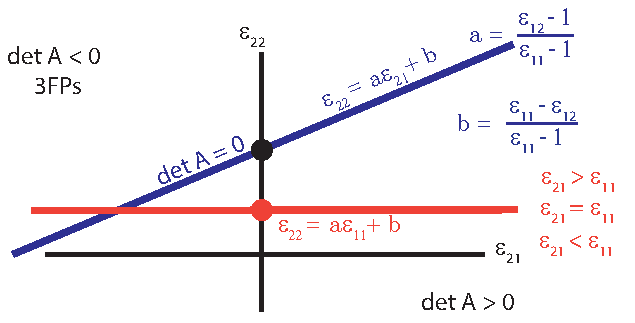
\includegraphics[width=\textwidth]{figures/bla_parameter_space}
  \caption{BLA parameter space.
}
  \label{fig:bla_parameter_space}
\end{figure}




\subsection{Fast-slow form}

We transform the state space so that the line attractor aligns with the $y$-axis.
So, we apply the affine transformation $R_\theta(x-\frac{1}{2})$ with the rotation matrix $R_\theta = \begin{bmatrix}\cos\theta &-\sin\theta\\\sin\theta&\cos\theta\end{bmatrix}= \begin{bmatrix}1 &1\\-1&1\end{bmatrix}$ where we have set $\theta=-\frac{\pi}{4}$.
So we perform the transformation $x\rightarrow x'= R_\theta(x-\frac{1}{2})$ and so we have $x=R^{-1}_\theta x'+\frac{1}{2}$ with $R^{-1}_\theta = R_{-\theta}$.
Then we get that 
\begin{align}
\dot x' = \operatorname{ReLU}\left(W(R^{-1}_\theta x'+\frac{1}{2})+1\right)-R^{-1}_\theta x'-\frac{1}{2}.
\end{align}
For a perturbation $W=\begin{bmatrix}\epsilon &-1\\-1&0\end{bmatrix}$ we get 
\begin{align}
\dot x' &= \operatorname{ReLU}\left(\begin{bmatrix}\epsilon &-1\\-1&0\end{bmatrix}\left(\begin{bmatrix}1 &-1\\1&1\end{bmatrix} x'+\frac{1}{2}\right)+1\right)-\begin{bmatrix}1 &-1\\1&1\end{bmatrix} x'-\frac{1}{2}\\
&=\begin{bmatrix}\epsilon-1 &-\epsilon-1\\-1&1\end{bmatrix}x' + \frac{1}{2}\begin{bmatrix}\epsilon-1 \\-1\end{bmatrix}+\begin{bmatrix}1 \\1\end{bmatrix}-\begin{bmatrix}1 &-1\\1&1\end{bmatrix} x'-\frac{1}{2}\begin{bmatrix}1 \\1\end{bmatrix}\\
&=\begin{bmatrix}\epsilon-2 &-\epsilon\\-2&0\end{bmatrix}x' + \frac{1}{2}\begin{bmatrix}\epsilon \\0\end{bmatrix}
\end{align}


Construct the fast-slow ODE as
\begin{align}
\dot y &= \epsilon y(y-1)(y+1) \\
\dot z &= -2z
\end{align}

\section{Heading direction network}

\begin{equation}
\tau \dot h_j = h_j + \frac{1}{N} \sum_k (W^{sym}_{jk} + v_{in} W^{asym}_{jk})\phi(h_k)+c_{ff},     j=1,\dots,N,
\end{equation}


\small

\bibliographystyle{plain}
\bibliography{cit.bib, CITCOD.bib, CITCom.bib}

\end{document}
